\documentclass[11pt,a4paper]{article}
\usepackage[utf8]{inputenc}
\usepackage[T1]{fontenc}
\usepackage{lmodern}
\usepackage[french]{babel}
\usepackage[margin=2.1cm]{geometry}
\usepackage{microtype}
\usepackage{amsmath,amssymb}
\usepackage{booktabs}
\usepackage{array}
\usepackage[table]{xcolor}
\usepackage{graphicx}
\usepackage{caption}
\usepackage[most]{tcolorbox}
\definecolor{navy}{HTML}{1F3864}
\definecolor{bluemid}{HTML}{2E5496}
\definecolor{lightblue}{HTML}{D6E0F0}
\captionsetup{font=small,labelfont={bf,color=navy},labelsep=period}
\graphicspath{{../figures/}}
\newtcolorbox{cle}[1][]{colback=lightblue!40,colframe=navy,boxrule=0.6pt,
  arc=2pt,left=8pt,right=8pt,top=6pt,bottom=6pt,#1}

\title{\vspace{-1.2cm}\color{navy}\bfseries Le déclenchement de P4 comme temps d'arrêt\\[2pt]
  \large L'extension dynamique du seuil $z^*$, et le raccord à la martingale}
\author{Kélian Kaddouri}
\date{27 juillet 2026}

\begin{document}
\maketitle
\vspace{-0.9cm}

\begin{cle}
\textbf{L'idée.} Le seuil de déclenchement de P4, $z^*=K_4/\sqrt{\rho}$, est jusqu'ici un niveau
statique du facteur tiers commun. Si ce facteur est un \textbf{processus} $Z_t$, le déclenchement
devient un \textbf{temps de premier passage} $\tau=\inf\{t:Z_t\ge z^*\}$, un \textbf{temps
d'arrêt}. Le \og{}moment\fg{} de déclenchement prend alors un sens temporel littéral, et le fil
rejoint le cadre martingale de l'identification.
\end{cle}

\medskip
\begin{center}
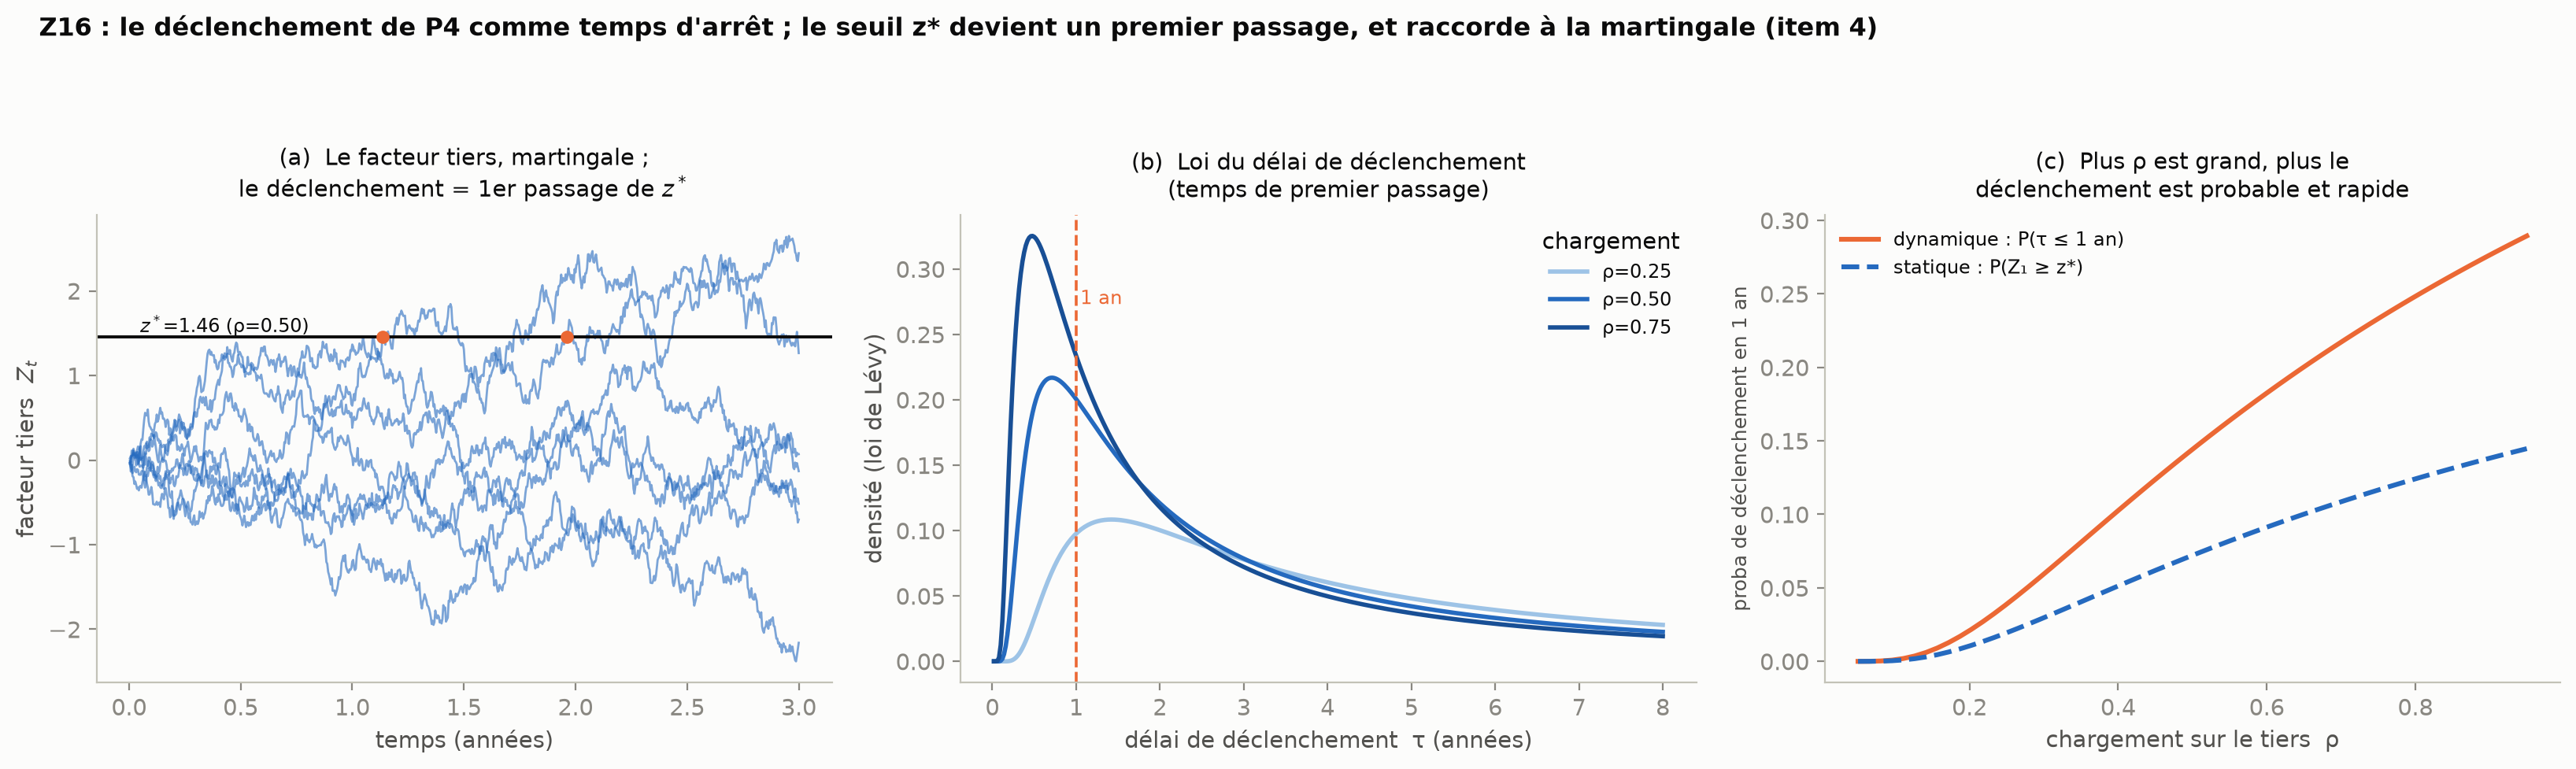
\includegraphics[width=\linewidth]{Z16_p4_temps_arret.png}
\captionof{figure}{\textbf{(a)} le facteur tiers (une martingale) et le premier passage de $z^*$.
\textbf{(b)} la loi du délai de déclenchement (temps de premier passage). \textbf{(c)} la lecture
dynamique $\mathbb{P}(\tau\le 1\text{ an})$ vaut environ le double de la statique.}
\end{center}

\noindent\textbf{Forme close.} Pour un mouvement brownien (une \textbf{martingale}), le principe
de réflexion donne
\[
  \mathbb{P}(\tau \le T) = 2\,\Phi\!\big(-z^*/\sqrt{T}\big),
\]
soit environ le double de la probabilité statique $\mathbb{P}(Z_T\ge z^*)$ : la lecture dynamique
compte tous les franchissements avant l'horizon, pas seulement la position finale. À $\rho=0{,}50$,
la probabilité de déclenchement de P4 en moins d'un an est $0{,}14$ (délai médian $\sim$5~ans) ;
à $\rho=0{,}75$, elle monte à $0{,}23$ (médian $\sim$3~ans). Plus le chargement sur le tiers est
grand, plus le déclenchement est probable \emph{et} rapide.

\begin{cle}
\textbf{Le fil se referme.} $Z_t$ sans dérive est une martingale et $\tau$ un temps d'arrêt : le
seuil de P4 rejoint ainsi le cadre \textbf{martingale} de l'identification ($W=S+A$ comme
réversibilité). Réserve assumée : le brownien pur atteint le niveau presque sûrement mais
d'espérance de délai infinie ; un facteur \textbf{moyen-réversif} (Ornstein-Uhlenbeck) donnerait
un taux de déclenchement récurrent fini, plus réaliste pour un facteur systémique. Le brownien
est le cas propre qui porte le lien théorique.
\end{cle}

\smallskip
\noindent\footnotesize\textcolor{navy}{\textbf{Source.}} Script
\texttt{6\_contagion/52\_p4\_temps\_arret.py}, figure \texttt{Z16\_p4\_temps\_arret.png}.
Prolonge le seuil $z^*$ (script~42) et raccorde à la note sur $W=S+A$ (script~40).

\end{document}
